\documentclass[12pt]{article}

\usepackage{sbc-template}
\usepackage{graphicx,url}
\usepackage{amssymb}
\usepackage{amsmath}
 \usepackage[sort&compress]{natbib}

\usepackage[brazil]{babel}   

\usepackage[utf8]{inputenc}
\sloppy

\title{Sugerindo colaborações na base de doutores da Plataforma Lattes usando Florestas Aleatórias}

\author{Gabriel Dahia, Gabriel L. P. e Souza, Pedro Vidal}

\address{Departamento de Ciência da Computação -- Universidade Federal da Bahia
  (UFBA)
  \email{\{gdahia,gabriellecomt,pvidal\}@dcc.ufba.br}
}

\begin{document} 

\maketitle

% TODO: abstract
% \begin{abstract}
%   This meta-paper describes the style to be used in articles and short papers
%   for SBC conferences. For papers in English, you should add just an abstract
%   while for the papers in Portuguese, we also ask for an abstract in
%   Portuguese (``resumo''). In both cases, abstracts should not have more than
%   10 lines and must be in the first page of the paper.
% \end{abstract}
     
% \begin{resumo} 
%   Este meta-artigo descreve o estilo a ser usado na confec��o de artigos e
%   resumos de artigos para publica��o nos anais das confer�ncias organizadas
%   pela SBC. � solicitada a escrita de resumo e abstract apenas para os artigos
%   escritos em portugu�s. Artigos em ingl�s dever�o apresentar apenas abstract.
%   Nos dois casos, o autor deve tomar cuidado para que o resumo (e o abstract)
%   n�o ultrapassem 10 linhas cada, sendo que ambos devem estar na primeira
%   p�gina do artigo.
% \end{resumo}


\section{Introdução}

A Plataforma Lattes, mantida pelo Conselho Nacional de Desenvolvimento Científico e Tecnológico (CNPq), corresponde à integração de bases de dados de Currículos, de Grupos de Pesquisa e de Instituições. Ela pauta atividades de planejamento e gestão, e a formulação de políticas públicas dos órgaos governamentais brasileiros~\cite{lattes-cnpq}.
Em especial, o Currículo Lattes foi criado pelo CNPq para centralizar, padronizar e disponibilizar, através da Plataforma Lattes, informações pessoais, profissionais e acadêmicas, fornecidas pelos próprios autores dos currículos, da comunidade científica brasileira~\cite{sucupira}.

Apesar da riqueza e potencial dessa base de dados, o CNPq impõe restrições ao acesso dessas informações, limitando o seu estudo.
Com intuito de disseminar o conteúdo da Plataforma Lattes, foi publicado o conjunto de dados \emph{LattesDoctoralDataset}.
Esta base contém dados a respeito do número e do tipo de publicações feitas, das colaborações entre pesquisadores, da atuação profissional e da formação acadêmica dos 265.187 doutores que possuem currículo publicado na plataforma~\cite{lattes-dataset}.

Ao analisar as colaborações entre doutores nesse banco de dados, é possível perceber que seu número é de aproximadamente 0,02\% do total possível.
Com o intuito de fomentar colaborações entre pesquisadores e, por consequência, o avanço da ciência no Brasil, esse trabalho propõe, analisando o \emph{LattesDoctoralDataset}, uma metodologia baseada em mineração de dados para sugerir novas colaborações com base nas informações fornecidas e nas colaborações preexistentes.

Usando Florestas Aleatórias~\cite{random-forests}, o método proposto atinge acurácia de $86,70\%~\pm~0,18$, com 99\% de confiança, quando a tarefa é: dado um par de currículos, determinar se há pelo menos uma colaboração entre esses pesquisadores.
Quando a tarefa é estimar o número de colaborações entre um par de pesquisadores, dados os seus currículos, o método consegue acurácia de $78,34\%~\pm~0,16$, com 99\% de confiança.

\section{Metodologia}
\label{sec:methods}

Para sugerir colaborações entre os doutores da base, primeiramente foi feito um pré-processamento na base de dados.
Este envolveu remover currículos com informações inconsistentes ou faltantes, agrupar as localizações e dados sobre a formação dos doutores, campos de preenchimento livre na Plataforma Lattes, utilizando técnicas de mineração de texto, e a remoção de atributos irrelevantes para a tarefa proposta.

Com a base pré-processada, o modelo empregado foi de Florestas Aleatórias, um conjunto de Árvores de Decisão treinado com diferentes partes da base de treino.

\subsection{Pré-processamento}
\label{sec:preprocess}

\begin{figure}
  \centering
  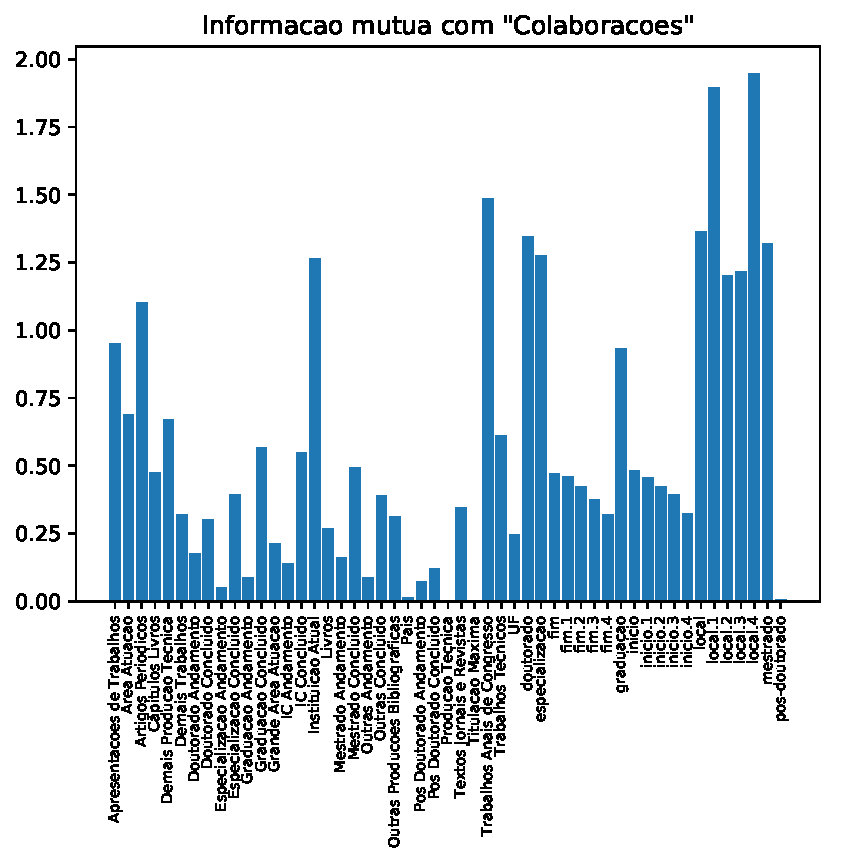
\includegraphics[width=0.45\textwidth]{graphs/mutual_information.pdf}
  \vspace{-15pt}
  \caption{Informação mútua de cada atributo com o atributo Colaborações para uma execução do método.}
  \label{fig:mutual-info}
\end{figure}

A base de dados \emph{LattesDoctoralDataset} contém 265.187 currículos, com informações sobre a atuação profissional, colaborações relatadas, produção científica, entre outros.
Para mais detalhes sobre a organização da base, sua coleta e conteúdo, o leitor interessado é referenciado ao artigo original de sua publicação~\cite{lattes-dataset}.

O primeiro passo do pré-processamento é o descarte de currículos que não tenham colaborações relatadas ou com informações faltantes.
Nessa etapa, todo currículo com valores inválidos nos campos de atuação profissional, e, excetuando o campo ``\texttt{pos-doutorado}'' e ``\texttt{especializacao}'', de formação acadêmica, são descartados.
Além disso, currículos que não tenham produção científica também são descartados, considerando que isto é um pré-requisito ao título de doutor.
Campos cujos significados não estão claros na especificação da base, como os de proficiência em línguas e os últimos campos da formação acadêmica, também foram descartados.

Os campos que podem ser especificados livremente no Currículo Lattes apresentam enorme variabilidade na maneira de especificar a mesma informação.
Por exemplo, no campo referente ao local de graduação, usuários podem especificar ``USP'', ``Universidade de São Paulo'' e ``Univ. de SP'' para se referir a mesma instituição.

Em dois conjuntos de campos a variabilidade se sobressai.
O primeiro deles, a que denominou-se \texttt{lugares}, consiste de todos os campos prefixados por ``\texttt{local}'' e o campo ``\texttt{Instituicao Atual}''.
O segundo, chamado de \texttt{formacao}, contém ``\texttt{doutorado}'', ``\texttt{graduacao}'', ``\texttt{especializacao}'', ``\texttt{mestrado}'' e ``\texttt{pos-doutorado}''.

Para mitigar os efeitos dessa variabilidade, utilizou-se Análise Semântica Latente (LSA)~\cite{lsa}.
Para isso, considerou-se cada entrada dos campos de ou \texttt{lugares}, ou \texttt{formacao}, a depender de qual conjunto está sendo agrupado, como um documento individual.
O resultado desse processo é a transformação dos valores desses campos em um vetores no espaço $\mathbb{R}^{100}$.
Em seguida, foi aplicado o algoritmo \emph{k-Means} para agrupar o conjunto de valores dos campos em 500 grupos, no caso de \texttt{formacao}, ou 3.000 grupos, no caso de \texttt{lugares}.
Este número foi calculado para comportar todas instituições de ensino superior no Brasil - 2.364, de acordo com~\cite{censo-mec} - e outras.

Depois desse agrupamento, calculou-se a produtividade de cada doutor como o total de colaborações relatadas; esse campo foi denominado ``\texttt{Colaboracoes}''.
Utilizando esse atributo como preditor da tarefa que se deseja resolver, calculou-se, entre todo outro atributo $X$ da base de dados e $Y = \texttt{Colaboracoes}$ a informação mútua $I$:
\begin{equation}
  I(X, Y) = \sum_{y \in Y} \sum_{x \in X} p(x, y) \log \left( \frac{p(x, y)}{p(x)p(y)} \right),
\end{equation}
onde $p(x, y)$ é a probabilidade conjunta de $X$ e $Y$, e $p(x)$ e $p(y)$ são, respectivamente, as probabilidades marginais de $X$ e $Y$.
$p(x)$, $p(y)$ e $p(x, y)$ são estimados, respectivamente, como as frequências empíricas de $x$ em $X$, $y$ em $Y$, e $(x, y)$ em $(X, Y)$.

Informalmente, $I(X, Y)$ quantifica quão independente as variáveis $X$ e $Y$ são; isso permite quantificar dependências lineares, como correlação é capaz de fazer, e não-lineares entre as distribuições estudadas.
A figura~\ref{fig:mutual-info} mostra os resultados.

Nessa etapa, todos os atributos independentes com ``\texttt{Colaboracoes}'' foram descartados do conjunto de dados.
O resultado foi uma versão da base de dados em que, em uma determinada execução, restaram 8.180 currículos restritos aos atributos não independentes de ``\texttt{Colaboracoes}''.
Nesta versão da base, existem 58.689 colaborações entre pesquisadores, em contraste com as 6.902.042 colaborações da base original.

% TODO: add figure illustrating the preprocessing pipeline

\subsection{Modelo de mineração de dados}
\label{sec:datamining}

O método de Florestas Aleatórias pode ser descrito da seguinte maneira: são construídos $N$ conjuntos de dados de tamanho igual ao da base original, através do sorteio com repetição dos exemplos do conjunto de dados inicial.
Em cada uma dessas novas bases, é treinada uma Árvore de Decisão.
O conjunto de todas essas árvores é o modelo de mineração de dados.

Para fazer inferência com esse modelo, são computadas as classes previstas por cada uma das árvores.
A predição final é obtida através do cálculo ou da média ou da moda das previsões individuais.

Esse modelo pode equivalentemente ser explicado como uso de \emph{bagging} para Árvores de Decisão.
Suas vantagens: são regularizar o modelo, diminuindo sobreajuste e aumentando a acurácia~\cite{random-forests}.

%Nesse trabalho, utilizou-se a implementação da biblioteca \emph{Scikit-learn}~\cite{sklearn} de Florestas Aleatórias, e limitou-se o número de árvores à 10; os outros parâmetros são mantidos os padrões especificados pela biblioteca.

\section{Experimentos}
\label{sec:experiments}

Como há estocasticidade no método a partir da etapa de pré-processamento, rodou-se o experimento 10 vezes com sementes aleatórias diferentes para cálculo de intervalos de confiança. 

Para cada execução individual do experimento, a base pré-processada foi dividida em um conjunto de treino, compreendendo 60\% do total de dados, e um conjunto de teste, com o restante.
A divisão é feita de maneira estratificada, considerando apenas se há ou não colaboração entre os donos dos currículos, isto é, são adicionadas colaborações existentes que são classificadas como o número de ocorrências da colaboração, e são adicionados um número igual de colaborações que não existem na base, classificadas como uma colaboração que nunca ocorreu.

O restante do experimento consiste em treinar um modelo de Floresta Aleatória no conjunto de treino e validá-lo no conjunto de teste em duas modalidades distintas, que denominou-se \texttt{binary} e \texttt{standard}.
A figura~\ref{fig:modalities} ilustra ambas modalidades.

\begin{figure}
  \begin{center}
    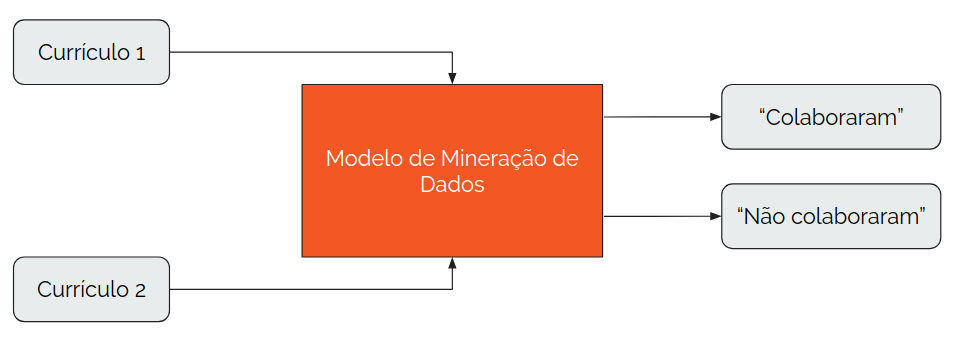
\includegraphics[width=0.45\textwidth]{images/binary.png}
    \hspace{10pt}
    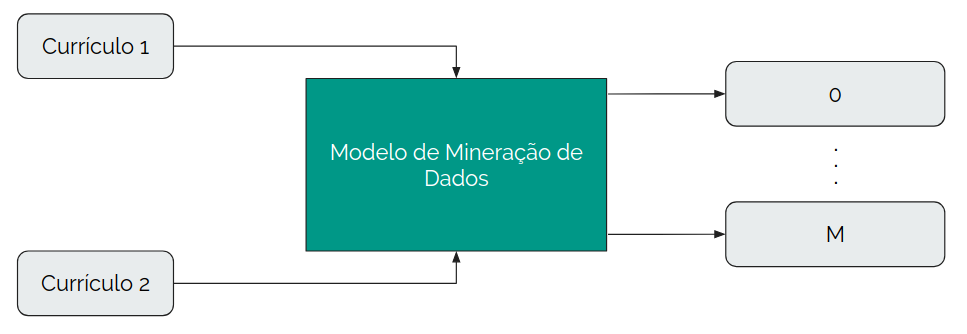
\includegraphics[width=0.45\textwidth]{images/standard.png}
  \end{center}
  \vspace{-15pt}
  \caption{Modalidades de mineração de dados: à esquerda, a modalidade \texttt{binary}, em que é necessário apenas determinar se há ou não colaboração entre os donos dos currículos. À direita, a modalidade \texttt{standard}, onde o par de currículos é classificado de acordo com o número de colaborações previsto.}
  \label{fig:modalities}
\end{figure}

Na modalidade \texttt{binary}, a tarefa consiste em determinar, dado um par de currículos, se há pelo menos uma colaboração entre eles.
Aqui, a Floresta Aleatória é treinada com pares de currículos como atributos e a informação de se há ou não colaboração entre eles como saída esperada.
Para fazer com que o modelo treinado seja robusto à ordem em que os currículos são colocados no par, duplicou-se o conjunto de treino, colocando currículos nos dois sentidos.

Já na modalidade \texttt{standard}, a tarefa consiste em estimar, dado um par de currículos, o número de colaborações entre eles.
Neste caso, o modelo é treinado com os pares de currículos e sua saída é uma classe de $\{0, 1, ..., M\}$, onde $M$ é o maior número de colaborações presente no conjunto de testes.

A validação do método usa a métrica acurácia, calculada como
\begin{equation}
  \textit{acurácia} = \frac{\text{Previsões corretas}}{\text{Total de previsões}}.
\end{equation}

Assim como é feito para o conjunto de treino, pares de currículos são também colocados nos dois sentidos no conjunto de teste.
Isso permite avaliar a robustez do método proposto à ordem em que os currículos são entregues ao modelo de mineração de dados sem artificialmente melhorar o resultado no conjunto de testes.

\subsection{Resultados}
\label{sec:results}
A partir das dez repetições do experimento, obteve-se $86,70\%~\pm~0,18$ de acurácia, com 99\% de confiança, para a modalidade \texttt{binary}, e $78,34\%~\pm~0,16$, com 99\% de confiança, para a modalidade \texttt{standard}.

Quando se compara estes resultados com a performance esperada de um classificador aleatório para essa mesma tarefa - dado que esta tarefa não foi tentada anteriormente e, portanto, não há estado-da-arte -, respectivamente 50\% para a modalidade \texttt{binary}, e 1,08\% (em média, existem 92 valores de colaborações possíveis) para a modalidade \texttt{standard}.

%É importante notar que o resultado apresentado, na verdade, se trata de um limite inferior para a performance do modelo no conjunto de teste.
%Isso ocorre porque, se para um determinado par de currículos para o qual foi previsto colaborações, não há colaboração relatada entre seus detentores, há três cenários possíveis: (1) realmente não há e nem nunca haverá colaboração entre esses pesquisadores e o modelo realmente fez uma classificação equivocada; (2) os doutores ainda não colaboraram, mas no futuro podem vir a colaborar; ou (3) há um erro no banco de dados e os doutores colaboraram, mas não relataram sua colaboração.
%Nos cenários (2) e (3), a acurácia calculada do modelo é inferior ao valor correto.
%Em especial, para o cenário (2), o \emph{LattesDoctoralDataset} não possui informação temporal e o modelo, portanto, não pode aprender esse tipo de informação.

Também é importante notar que a discrepância nos resultados entre as modalidades pode ser explicada pelo fato de a tarefa proposta para \texttt{standard} ser consideravelmente mais difícil do que a de \texttt{binary}: é possível que um dado número de colaborações não apareça no treino e todas as instãncias dessa classe seriam mal-classificadas.
Além do mais, a avaliação proposta não considera a proximidade do número de colaborações previsto do real; apenas previsões corretas são consideradas.

Apesar do grande número de nós em cada árvore (aproximadamente 20 mil), é possível realizar inferência no modelo, uma vez carregado em memória principal, em tempo real.
Isso ocorre porque a altura é, no máximo, o número de atributos fornecidos ao modelo, que não passa de 100. % em media, sao 96 atributos
Além disso, os arquivos dos modelos têm tamanho razoável: aqueles para a modalidade \texttt{binary} têm em torno de 15MB, e os \texttt{standard} têm em torno de 250MB.

% TODO: maybe daniela will complain about not comparing to similar works for other datasets, we can argue that in the specs, review is not listed. the limit of pages can also be listed as an argument. we can also use this excuse to say adjsutments to the text are required, prior to publication and stall it

\section{Conclusão}
\label{sec:conclusion}

Esse trabalho apresentou um modelo de mineração de dados baseado em Florestas Aleatórias capaz de prever colaborações entre doutores da base \emph{LattesDoctoralDataset}.
Além de estabelecer resultados iniciais para essa base, a acurácia obtida mostra que esse sistema é preciso o suficiente para ser utilizado na prática, sem problemas com tempo de execução ou requisito de armazenamento.

Foram identificadas, contudo, limitações da metodologia proposta que podem ser melhoradas em versões futuras.
O tratamento de dados faltantes ou fora de conformação pode ser melhorado já que atualmente consiste em eliminar instâncias com erros detectáveis e mineração de texto para os campos de preenchimento livre.

A abordagem de mineração de textos empregada, inclusive, não generaliza caso haja termos não presentes no conjunto de dados analisado - também imagina-se que um método de mineração de textos mais robusto que LSA possa melhorar os resultados.

Melhores resultados também devem poder ser obtidos integrando o processo de colheita de uma nova versão da base de dados com as demandas do modelo de aprendizado de máquina.
Como mencionado anteriormente, maior padronização das informações e a informação temporal das colaborações pode melhorar a performance da metodologia.

 \setlength{\bibsep}{0ex}
\vspace{-5pt}
\bibliographystyle{sbc}
\bibliography{refs}

\end{document}
